%%%%%%%%%%%%%%%%%%%%%%%%%%%%%%%%%%%%%%%%%%%%%%%%%%%%%%%%%%%%%%%%%%%%%%%%%%%%%%%%
% Version Control Systems
%
% Author: FOSSEE 
% Copyright (c) 2009, FOSSEE, IIT Bombay
%%%%%%%%%%%%%%%%%%%%%%%%%%%%%%%%%%%%%%%%%%%%%%%%%%%%%%%%%%%%%%%%%%%%%%%%%%%%%%%%

\documentclass[14pt,compress]{beamer}

\mode<presentation>
{
  \usetheme{Warsaw}
  \useoutertheme{infolines}
  \setbeamercovered{transparent}
}

\usepackage[english]{babel}
\usepackage[latin1]{inputenc}
%\usepackage{times}
\usepackage[T1]{fontenc}

% Taken from Fernando's slides.
\usepackage{ae,aecompl}
\usepackage{mathpazo,courier,euler}
\usepackage[scaled=.95]{helvet}

\definecolor{darkgreen}{rgb}{0,0.5,0}

\usepackage{listings}
\lstset{language=bash,
    basicstyle=\ttfamily\bfseries,
    commentstyle=\color{red}\itshape,
  stringstyle=\color{darkgreen},
  showstringspaces=false,
  keywordstyle=\color{blue}\bfseries}

\begin{document}

\begin{frame}

\begin{center}
\vspace{12pt}
\textcolor{blue}{\huge Using Linux Tools}
\end{center}
\vspace{18pt}
\begin{center}
\vspace{10pt}

\includegraphics[scale=0.95]{../images/fossee-logo.png}\\
\vspace{5pt}
\scriptsize Developed by FOSSEE Team, IIT-Bombay. \\ 
\scriptsize Funded by National Mission on Education through ICT\\
\scriptsize  MHRD,Govt. of India\\

\includegraphics[scale=0.30]{../images/iitb-logo.png}\\
\end{center}
\end{frame}

\begin{frame}
  \frametitle{Objectives}
  At the end of this session, you will be able to:
  \begin{itemize}
  \item Understand what is Version Control and the need for it.
  \item Create and use repository on a daily basis.
  \end{itemize}
\end{frame}

%% There are some %$ used just to minimise the effect of $ sign used
%% in lstlisting. In emacs it looks dirty. 

% Introduction to course-need of version control, history, options available.
\section{Introduction}

\begin{frame}
  \frametitle{What is Version Control?}
  \begin{block}{}
    A way to track changes made to files over time, by keeping copies
    of files as we change them.
  \end{block}
\end{frame}

%% Home made version control system?
\begin{frame}[fragile]
  \frametitle{Home-brewed}
  \begin{center}
    An example of a \typ{home-brew} Version Control system
    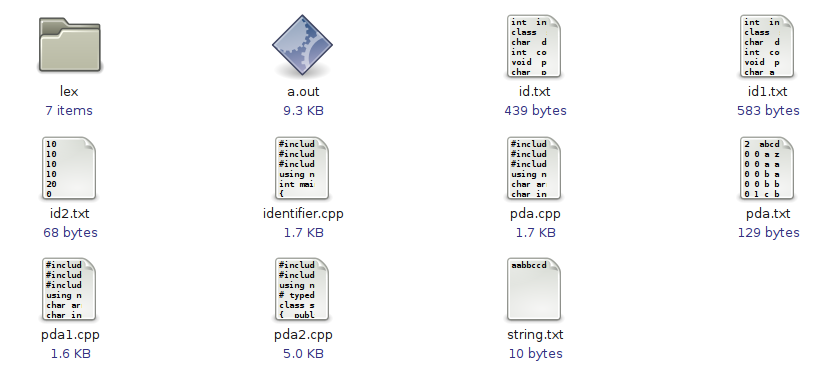
\includegraphics[height=1.8in,width=4.2in]{images/folder.png}
  \end{center}
  \begin{lstlisting} 
$ ls
a.out  id1.txt  id2.txt  identifier.cpp  id.txt  lex  pda1.cpp  pda2.cpp  pda.cpp  pda.txt  string.txt
  \end{lstlisting} %%$
    %%a screen-shot of folder with all crazy names.
\end{frame}

\begin{frame}[fragile]
  \frametitle{Problems}  
  \begin{block}{}    
  \begin{itemize}
  \item Name and changes made are not related or linked. 
  \item Can't track sequence of changes made to a file. 
  \item Does not scale. 
  \end{itemize}
    \end{block}
\end{frame}

\begin{frame}[fragile]
  \frametitle{The need for Version Control}
  \begin{itemize}
  \item \alert{To err is Human} \ldots 
  \item Tracking the history and evolution of a project
  \item To collaborate effectively on a project
  \item To efficiently track down bugs and pin-point the changes that
    caused it 
  \end{itemize}
\end{frame}

%% Introduction to how logs are managed in VCS.
%% A analogy in logs and day-to-day life?
\begin{frame}[fragile]
  \frametitle{How does it work? --- Analogy}
  It is, in some ways, similar to playing an Video game.
  \begin{itemize}
  \item We play games in stages
  \item Once we finish a stage or a task -- \alert{we SAVE}
  \item We continue playing
  \item But, if necessary, we could choose from one of the saved
    states and start from there
  \item We could alter the course of the game
  \end{itemize}
\end{frame}


\begin{frame}
  \frametitle{Mercurial or \typ{hg}}
  \begin{center}
    
\includegraphics[height=.75in,interpolate=true]{images/mercurial_logo}
  \end{center}
  \begin{itemize}
  \item Easy to learn and use
  \item Lightweight
  \item Scales excellently
  \item Written in Python
  \end{itemize}
\end{frame}

\begin{frame}
  \frametitle{Installation}
  \begin{itemize}
  \item \typ{sudo apt-get install mercurial}
  \item TortoiseHg
  \item \typ{\$ hg}
  \item \typ{\$ hg version}
  \end{itemize}
\end{frame}

\section{Let there be a Repo!}
% init, status, commit, log, [ui]
\begin{frame}
  \frametitle{We need a repo!}
  \begin{itemize}
  \item A Repository (repo) is where all the action is!
  \item Project files along with a special directory that stores all the
    changes
  \item We take snapshots of the whole repository; not individual
    files. 
  \end{itemize}
\end{frame}

\begin{frame}
  \frametitle{Initializing a repo}
  \begin{itemize}
  \item \typ{\$ hg init}
  \item Creates a fresh repository
  \item Adds a \typ{.hg} directory to our \emph{working directory}
  \end{itemize}
  \emphbar{\typ{.hg} directory keeps log of changes made henceforth}
\end{frame}

\begin{frame}
  \frametitle{Status report}
  \begin{itemize}
  \item \typ{hg status} gives the status of our repo
  \item Use it often; at least as a beginner
  \item \typ{hg help command} gives us help about \typ{command}
  \end{itemize}
\end{frame}

\begin{frame}[fragile]
  \frametitle{Status codes}
  \begin{lstlisting}
    M = modified                                               
    A = added                                                  
    R = removed                                                
    C = clean                                                  
    ! = missing 
    ? = not tracked                                            
    I = ignored                                                
  \end{lstlisting}
\end{frame}

\begin{frame}
  \frametitle{Adding files}
  \begin{itemize}
  \item From \typ{hg status} we know, none of the files are being
    tracked, yet. 
  \item \typ{hg add} --- asking \typ{hg} to track these files
  \item As expected \typ{hg status} prepends an \typ{A} to the file
  names.
  \item \typ{? --> A} 
  \item \typ{! --> R} (\typ{hg remove})
  \end{itemize}
\end{frame}

\begin{frame}
  \frametitle{Taking Snapshots}
  \begin{itemize}
  \item \typ{hg commit}
  \item Asking Mercurial to take a snapshot; remember the changes made
    to the repository. 
  \item \typ{-u FirstName LastName <email>}
  \item \typ{-m ``Commit message''} -- a description of changes committed. 
  \end{itemize}
\end{frame}

\begin{frame}
  \frametitle{Thumbnail views}
  \begin{itemize}
  \item \typ{hg log}~ gives the log of the changes made
  \item A \typ{changeset} is an atomic collection of changes to the
    files (between successive commits)
  \end{itemize}
  \begin{block}{Log information}
    \begin{itemize}
    \item \alert{changeset}: Identifier for the changeset
    \item \alert{user}: Details of user who created the changeset
    \item \alert{date}: Date and time of creation
    \item \alert{summary}: One line description
    \end{itemize}    
  \end{block}
\end{frame}

\begin{frame}
  \frametitle{User information}
  \begin{itemize}
  \item User information is set in the \typ{hgrc} file
  \item It can be set globally or local to the project
  \item Global \typ{hgrc}
    \begin{itemize}
    \item \typ{\$HOME/.hgrc} -- Unix like systems
    \item \typ{\%HOME\%\\.hgrc} -- Windows
    \end{itemize}
  \end{itemize}
\end{frame}

\begin{frame}
  \frametitle{\alert{Advice}: \typ{commits}, messages}
  \begin{itemize}
  \item Atomic changes; one change with one \typ{commit}
  \item Single line summary --- 60 to 65 characters long
  \item Followed by paragraphs of detailed description
    \begin{itemize}
    \item Why the change?
    \item What does it effect?
    \item Known bugs/issues?
    \item etc. 
    \end{itemize}
  \end{itemize}
\end{frame}

\begin{frame}
\frametitle{Summary}
\label{sec-8}

  In this tutorial, we have learnt to,


\begin{itemize}
\item 
\item 
\item 
\item 
\end{itemize}
\end{frame}
\begin{frame}[fragile]
\frametitle{Evaluation}
\label{sec-9}


\begin{enumerate}
\item 
\item 
\item 
\end{enumerate}
\end{frame}
\begin{frame}
\frametitle{Solutions}
\label{sec-10}


\begin{enumerate}
\item 
\vspace{15pt}
\item 
\end{enumerate}
\end{frame}
\begin{frame}

\begin{block}{}
  \begin{center}
  \textcolor{blue}{\Large THANK YOU!} 
  \end{center}
  \end{block}
\begin{block}{}
  \begin{center}
    For more Information, visit our website\\
    \url{http://fossee.in/}
  \end{center}  
  \end{block}
\end{frame}

\end{document}
